\section{Setup}\label{sc:setup}
To test our original scenario described in the Introduction on page \pageref{ch:introduction} we built a smaller version of the running track. To get a constant speed and a track to run tests on we use a Brio\texttrademark train to symbolism a human runner that runs a track. The speed of the runner was set to $12\dfrac{km}{hr}$ but the Brio train had a speed of $0.2604\dfrac{km}{hr}$. The track we used in the theory part was 906.17m long and the runner would run a marathon which is 46.56km and therefor is 46.56 rounds. Using the standard Brio track pack we build a track with length of 43.5cm. In the theory we send $4\dfrac{packets}{sec}$ so we needed to account for the differences between our test setup and the theory made in section \ref{table:datascenarios} on page \pageref{table:scenarios}.





 and 56cm. 


\begin{figure}[H]
	\centering
	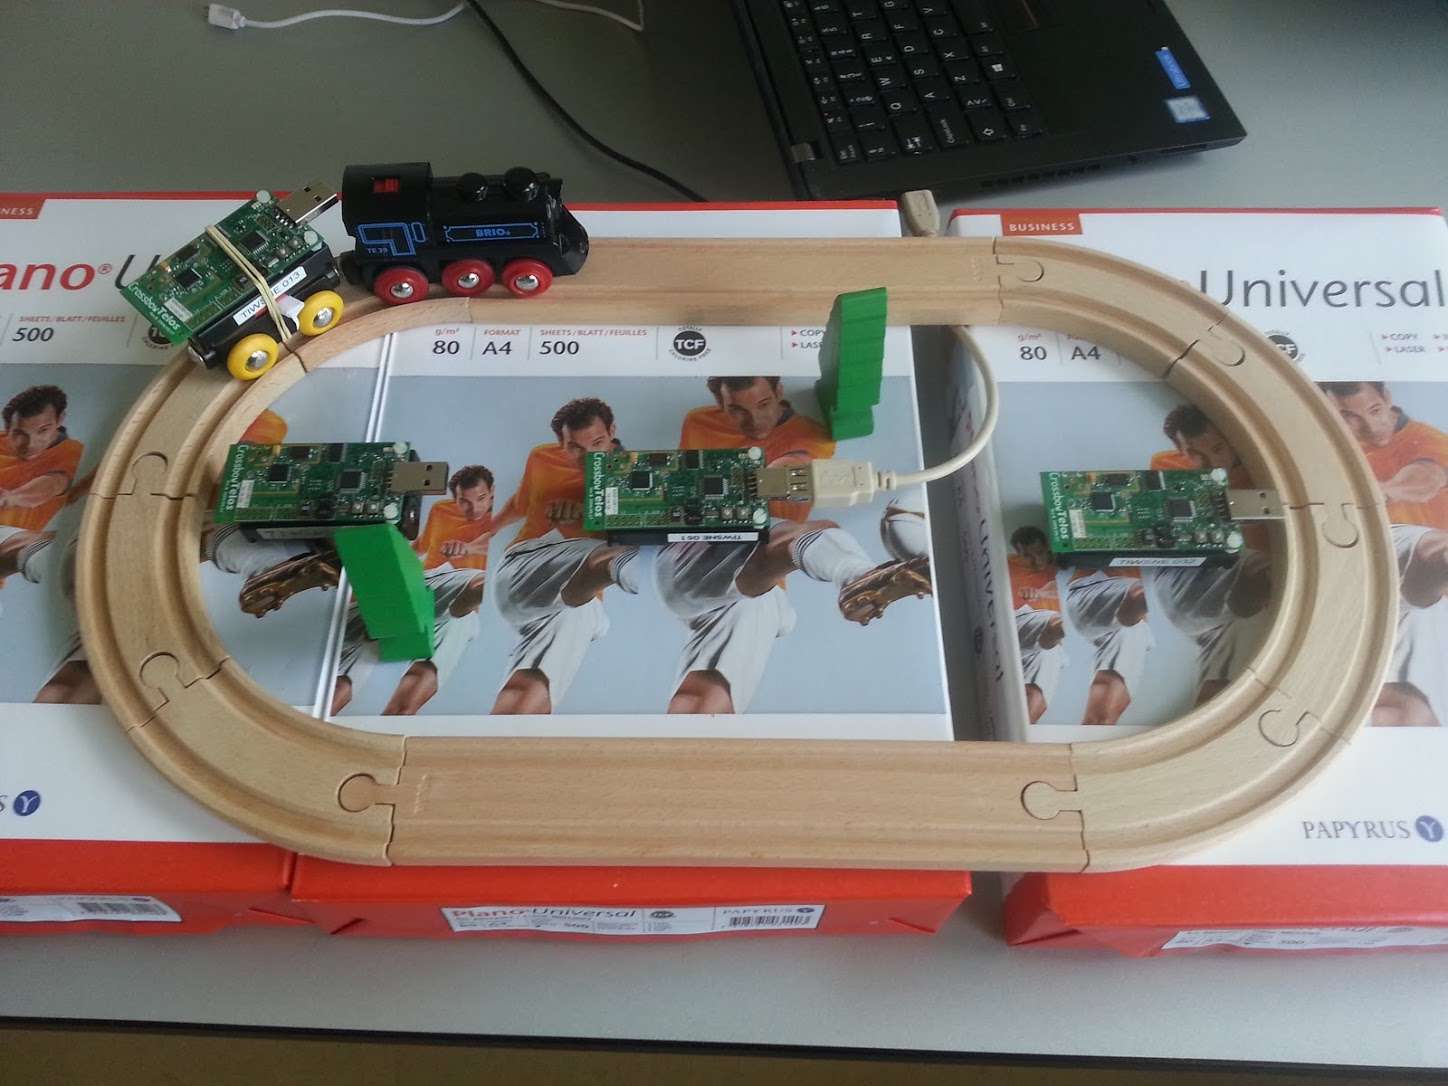
\includegraphics[width=1\linewidth]{testAndPerformance/setup/setup}
	\caption{The train track withbasestation, north and south relay nodes and the runner. }
	\label{fig:testSetup}
\end{figure}

